\documentclass{rvcepaper}
\begin{document}

% ---------- HS261TA Principles of Management and Economics
\begin{iempaper}
\paperinfo{date={28\textsuperscript{th} April 2025},exam={CIE -- I},maxmarks={10 + 50},sem={VI},prog={UG},duration={30 + 90 Min},
 title={Principles of Management and Economics},code={HS261TA}}
\iemhead
\begin{cietable}{M}{BT}{CO}
\qpart{Part -- A}
\q{1}{Mention any two skills required by an effective manager.}{2}{L1}{01}
\q{2}{List any two principles of scientific management as proposed by F W Taylor.}{2}{L1}{01}
\q{3}{Highlight the importance of Hawthorne Studies.}{2}{L2}{01}
\q{4}{Differentiate between micro and macroeconomics.}{2}{L2}{04}
\q{5}{What are the two main sectors in a simple circular flow model?}{2}{L1}{05}
\qpart{Part -- B}
\q{1}{A retail chain wants to optimize its store operations for better customer service and efficiency. How can the principles of Scientific Management and Administrative Theory help in this scenario?}{10}{L3}{01}
\q{2}{You are part of the organizing committee for a Techno-Cultural Fest at your institution. Apply the five primary functions of management---Planning, Organizing, Staffing, Directing, and Controlling---to successfully manage the event. Explain how each function can be implemented to ensure the fest runs smoothly and meets its objectives.}{10}{L3}{01}
\q{3}{A large multinational company is facing challenges in managing its various departments and adapting to changes in the external market environment. Apply \textbf{Systems Theory} and \textbf{Contingency Theory} to suggest how the company can improve its overall management and operations. Explain how these theories would help in managing the complexity and adapting to the changing conditions.}{10}{L4}{01}
\q{4}{Consider an economy that is experiencing high inflation and high unemployment simultaneously (stagflation). Using the Circular Flow Model of Economics, explain how inflation and unemployment are interconnected in this economy. How can government policies in the form of fiscal and monetary interventions help address these issues?}{10}{L4}{04}
\q{5}{A country is transitioning from a command economy to a market economy. Using an overview of Economic Systems, discuss the potential advantages and disadvantages of this shift.}{10}{L2}{05}
\end{cietable}
\end{iempaper}

% ---------- IM362IA Supply Chain Management
\begin{iempaper}
\paperinfo{date={28\textsuperscript{th} April 2025},exam={CIE -- I},maxmarks={10 + 50},sem={VI},prog={UG},duration={30 + 90 Min},
 title={Supply Chain Management},code={IM362IA}}
\iemhead
\begin{cietable}{M}{BT}{CO}
\qpart{Part -- A}
\q{1.}{List the processes under SRM -- macro process.}{2}{1}{CO1}
\q{2.}{Sketch the implied uncertainty (demand and supply) spectrum and cite examples.}{2}{2}{CO1}
\q{3.}{Compare Efficient and Responsive Supply Chains(any two).}{2}{1}{CO1}
\q{4.}{Mention any two challenges to achieving and maintaining strategic fit.}{2}{1}{CO1}
\q{5.}{Illustrate the relationship between desired response time and number of facilities.}{2}{2}{CO2}
\qpart{Part -- B}
\q{1}{Identify the five stages of a supply chain and sketch four process cycles. Explain the sub-processes in a supply chain process cycle of your choice for a manufacturing supply chain.}{10}{3}{CO1}
\q{2}{Illustrate and analyse the value chain for a manufacturing organisation.}{10}{3}{CO1}
\q{3}{Evaluate the various stages involved in expanding the scope of strategic fit for an automobile supply chain.}{10}{3}{CO1}
\q{4}{Discuss the role that information plays in the supply chain, as well as key information-related decisions that supply chain managers must make.}{10}{2}{CO1}
\q{5}{Select the supply chain of your choice evaluate the performance of a distribution network along two dimensions: Customer needs that are met (service); and Cost of meeting customer needs.}{10}{4}{CO2}
\end{cietable}
\end{iempaper}

% ---------- IM363IA Ergonomics
\begin{iempaper}
\paperinfo{date={29\textsuperscript{th} April 2025},exam={CIE -- I},maxmarks={10 + 50},sem={VI},prog={UG},duration={30 + 90 Min},
 title={ERGONOMICS},code={IM363IA}}
\iemhead
\begin{cietable}{M}{BT}{CO}
\qpart{Part -- A}
\q{1.}{Define human factors engineering in one sentence.}{01}{L1}{CO1}
\q{2.}{Name any two objectives of ergonomics.}{01}{L2}{CO1}
\q{3.}{What is meant by user-centred design?}{01}{L2}{CO2}
\q{4.}{Mention one example of cognitive ergonomics in interface design.}{01}{L1}{CO2}
\q{5.}{List the three types of anthropometric data.}{01}{L1}{CO2}
\q{6.}{What does percentile mean in the context of anthropometric measurements?}{01}{L2}{CO2}
\q{7.}{State one principle of workspace design for sitting tasks.}{01}{L1}{CO3}
\q{8.}{What is the primary goal of ergonomics in design?}{01}{L1}{CO2}
\q{9.}{Differentiate between static and dynamic anthropometry with one word each.}{01}{L2}{CO2}
\q{10.}{Which part of the body is most commonly associated with low back pain due to poor workspace ergonomics?}{01}{L2}{CO3}
\qpart{Part -- B}
\q{1.}{Develop a step-by-step ergonomic evaluation plan for a manufacturing workstation. Your answer should include: Identification of key task elements, Application of anthropometric measurements, Postural analysis methods, Recommendations to reduce musculoskeletal risks.}{10}{L3}{CO1}
\q{2.}{Analyze the causes of work-related musculoskeletal disorders (WMSDs) in the context of poor workspace design. Use the following structure: Ergonomic risk factors, Examples of bad design, Physiological consequences on the musculoskeletal system, Suggestions for redesign based on anthropometry.}{10}{L4}{CO3}
\q{3.}{A company is designing a standing workbench for both male and female operators in an electronics assembly line. Apply anthropometric principles to determine optimal workbench height, Analyze how human variability influences design decisions, Discuss trade-offs between productivity, comfort, and injury prevention.}{10}{L4}{CO2}
\q{4.}{The 97.5th percentile value and 2.5\textsuperscript{th} percentile values of normally distributed variable is found by adding/subtracting 1.96 standard deviation from the mean. If the mean body mass of males of a certain populations is 82.1 Kg and the standard deviation is 17.1 kg, what are the 2.5th percentile value and the 97.5th percentile values? How will use the results of this calculation be used in considering the range of users covered in design?}{10}{L4}{CO2}
\q{5.}{Discuss the scope of work that is covered under the following type of ergonomic studies.
\begin{romi}
\item Physical ergonomics.
\item Cognitive ergonomics.
\item Organizational ergonomics.
\item Macro ergonomics.
\end{romi}}{10}{L2}{CO1}
\end{cietable}
\end{iempaper}

% ---------- IM364TA Human Resource Management & Analytics
\begin{iempaper}
\paperinfo{date={29\textsuperscript{th} April 2025},exam={CIE -- I},maxmarks={10 + 50},sem={VI},prog={UG},duration={30 + 90 Min},
 title={Human Resource Management \& Analytics -- IM364TA},code={}}
\noindent\hspace*{0pt}
\begin{center}{\fontsize{12}{14}\selectfont DEPARTMENT OF}\\[3pt]{\bfseries\fontsize{15.5}{18}\selectfont INDUSTRIAL ENGINEERING \& MANAGEMENT}\end{center}\vspace{-3pt}
\noindent\begingroup\renewcommand{\arraystretch}{2.0}\bfseries\fontsize{11.5}{13}\selectfont
\begin{tabular}{|p{6.2cm}|C{5.0cm}|p{5.5cm}|}\hline
 Date \hspace{0.5cm}: \hspace{0.2cm}29\textsuperscript{th} April 2025 & CIE -- I & Max. Marks \hspace{0.3cm}: \hspace{0.2cm}10 + 50\\\hline
 Semester \hspace{0.1cm}: \hspace{0.2cm}VI & UG & Duration \hspace{0.55cm}: \hspace{0.2cm}30 + 90 Min\\\hline
 \multicolumn{3}{|C{16.7cm}|}{Human Resource Management \& Analytics - IM364TA}\\\hline
\end{tabular}\endgroup\par\vspace{4pt}
\iemnote
\begin{cietable}{M}{BT}{CO}
\qpart{Part -- A}
\q{1.}{What is Talent Management?}{02}{L1}{CO1}
\q{2.}{List the type of information that can be collected through job analysis.}{02}{L2}{CO1}
\q{3.}{List the three steps in Succession planning.}{02}{L2}{CO1}
\q{4.}{Differentiate between Job specification and Job description.}{02}{L1}{CO1}
\q{5.}{Name the main internal sources of candidates.}{02}{L2}{CO2}
\qpart{Part -- B}
\q{1}{Bright Minds School hired a new HR Manager, Ms. Riya, to transform its HR practices. While she has excellent knowledge of HR policies, she faces challenges in communication, conflict resolution, and strategic thinking. The management is unsure if she is the right fit for a role that requires leadership and organizational development.\newline
\textbf{Questions:}
\begin{num}
\item Based on this case, identify which HR competencies are lacking and how these gaps can affect HRM outcomes.
\item Suggest ways Ms. Riya can develop the necessary competencies to succeed in her role.
\item Discuss how aligning HR objectives with organizational goals can enhance overall institutional effectiveness in this context.
\end{num}}{10}{L4}{CO1}
\q{2}{Imagine you are working in the HR department of a delivery company called SwiftCart Logistics. The company needs a clear job profile for the role of Delivery Executive to improve hiring and performance. Write the a) Job Description for the role of Delivery Executive and b) Job Specification for the same role.}{10}{L3}{CO1}
\q{3}{Name any four methods used for collecting Job Analysis information for roles like cashier.}{10}{L3}{CO1}
\q{4}{Mention two internal and two external sources of recruitment for roles like chefs. Provide one example for each.}{10}{L3}{CO2}
\q{5}{Ritz Resort is expanding its operations and requires new hires for key positions such as spa therapists, chefs, and front desk receptionists. The HR department is in charge of managing the entire recruitment process to ensure the right candidates are selected quickly and effectively.\newline
Questions:
\begin{num}
\item Describe the key steps in the recruitment process that the HR team at Ritz Resort should follow when hiring spa therapists and chefs.
\item How can they ensure the quality of candidates selected for these roles?
\end{num}}{10}{L4}{CO2}
\end{cietable}
\stars{----- * * * -----}
\end{iempaper}

% ---------- IM365TDA Facilities Planning and Design
\begin{iempaper}
\paperinfo{date={02\textsuperscript{nd} May 2025},exam={CIE -- I},maxmarks={10 + 50},sem={VI},prog={UG},duration={30 + 90 Min},
 title={Facilities Planning and Design},code={IM365TDA}}
\iemhead
\begin{cietable}{M}{BT}{CO}
\qpart{Part -- A}
\q{1.}{Facilities planning are subdivided into the subjects of facilities \blank[1.9cm] and facilities \blank[1.9cm].}{(02)}{L1}{CO1}
\q{2.}{State two objectives of facilities planning.}{(02)}{L2}{CO1}
\q{3.}{List two factors of facilities location.}{(02)}{L1}{CO1}
\q{4.}{Expand CRAFT and COFAD.}{(02)}{L1}{CO1}
\q{5.}{What is the basic principle of the CORELAP algorithm, and how is the first department selected?}{(02)}{L1}{CO1}
\qpart{Part -- B}
\q{1.}{Enumerate and analyse the characteristics of all the facilities of a supply chain to achieve excellence.}{10}{L2}{CO1}
\q{2.}{Apply the Winning facilities planning process methodology for facilities planning of a manufacturing organization, and provide your analysis summary.}{10}{L3}{CO3}
\q{3.}{Perform a comparative assessment of the performance characteristics of process layout, product layout and cellular layout.}{10}{L2}{CO2}
\q{4.}{An Auto Parts warehouse has requested that a new layout be designed for their main warehouse. The warehouse has 8 major activity centers. The current building area can accommodate 10 X 24 unit squares. Develop the new layout using ALDEP using the data given below.
\par\vspace{4pt}\centerline{\begin{tabular}{|C{1.6cm}|l|C{2.6cm}|}\hline \textbf{Code} & \textbf{Department Name} & \textbf{Area (m\textsuperscript{2})}\\\hline 1 & Storage & 12800\\\hline 2 & Counter & 8800\\\hline 3 & Paint Room & 9200\\\hline 4 & Receiving & 12000\\\hline 5 & Office & 8800\\\hline 6 & Parts Bins & 13200\\\hline 7 & Tailpipe Racks & 13200\\\hline 8 & Restroom & 8000\\\hline\end{tabular}}\par\vspace{4pt}
\par\noindent\begin{tabular}{|C{0.8cm}|C{0.8cm}|C{0.8cm}|C{0.8cm}|C{0.8cm}|C{0.8cm}|C{0.8cm}|C{1.7cm}|}\hline
1 & \multicolumn{7}{c|}{-------}\\\hline
2 & X & \multicolumn{6}{c|}{-------}\\\hline
3 & O & O & \multicolumn{5}{c|}{-------}\\\hline
4 & A & X & U & \multicolumn{4}{c|}{-------}\\\hline
5 & U & E & U & U & \multicolumn{3}{c|}{-------}\\\hline
6 & O & A & O & U & U & \multicolumn{2}{c|}{-------}\\\hline
7 & O & I & I & U & U & I & -------\\\hline
8 & O & O & O & U & O & O & O\\\hline\end{tabular}\par\vspace{4pt}
\centerline{\begin{tabular}{|l|C{1.2cm}|C{1.2cm}|C{1.2cm}|C{1.2cm}|C{1.2cm}|C{1.4cm}|}\hline Closeness Value & A & E & I & O & U & X\\\hline & 64 & 16 & 4 & 1 & 0 & -1024\\\hline\end{tabular}}\par\vspace{4pt}
Minimum Department Preference (MDP) = I = 4, Sweep Width = 2, Number of iterations to be performed, N = 3, Assume Scale: 1 square = 400 m2, Length X Width for the layout: 10 X 24}{10}{L3}{CO3}
\q{5.}{Given the initial layout, flow matrix and cost matrix shown in figures 1,2 and 3, use the CRAFT scoring method and procedure two ways to obtain an improved layout.(consider any two possible exchanges).
\par\vspace{4pt}\noindent\begin{minipage}[c]{4.6cm}\centering
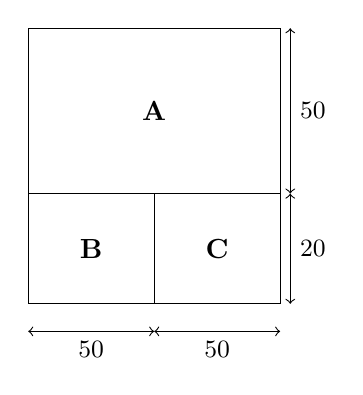
\begin{tikzpicture}[x=0.032cm,y=0.07cm]\draw (0,0) rectangle (100,50);\draw (0,0) rectangle (50,20);\draw (50,0) rectangle (100,20);\draw (0,20) rectangle (100,50);
\node at (50,35) {\bfseries A};\node at (25,10) {\bfseries B};\node at (75,10) {\bfseries C};
\draw[<->] (104,20)--(104,50);\node[right] at (104,35) {\small 50};\draw[<->] (104,0)--(104,20);\node[right] at (104,10) {\small 20};
\draw[<->] (0,-5)--(50,-5);\node[below] at (25,-5) {\small 50};\draw[<->] (50,-5)--(100,-5);\node[below] at (75,-5) {\small 50};\end{tikzpicture}\\[10pt]{\small Fig 1. Initial Layout}\end{minipage}\hspace{0.3cm}%
\begin{minipage}[c]{4.6cm}\centering\renewcommand{\arraystretch}{1.25}\begin{tabular}{|c|c|c|c|}\hline From $\backslash$ To & A & B & C\\\hline A & & 4 & 1\\\hline B & 2 & & 2\\\hline C & 2 & 1 & \\\hline\end{tabular}\\[6pt]{\small Fig. 2. Flow Matrix}\end{minipage}\hspace{0.3cm}%
\begin{minipage}[c]{4.6cm}\centering\renewcommand{\arraystretch}{1.25}\begin{tabular}{|c|c|c|c|}\hline From $\backslash$ To & A & B & C\\\hline A & & 1 & 1\\\hline B & 1 & & 1\\\hline C & 1 & 1 & \\\hline\end{tabular}\\[6pt]{\small Fig. 3 Cost Matrix}\end{minipage}}{10}{L1}{CO1}
\end{cietable}
\stars{*****}
\end{iempaper}

% ---------- IM365TDB Service Operations Management
\begin{iempaper}
\paperinfo{date={2\textsuperscript{nd} May 2025},exam={CIE -- 1},maxmarks={10 + 50},sem={VI},prog={UG},duration={30 + 90 Min},
 title={Service Operations Management},code={IM365TDB}}
\iemhead
\begin{cietable}{M}{BT}{CO}
\qpart{Part -- A}
\q{1.}{What is the primary goal of Service Operations Management?}{2}{1}{1}
\q{2.}{Name two major challenges faced by service operations managers in today's dynamic environment.}{2}{2}{2}
\q{3.}{Differentiate between B2B and B2C services with one example each.}{2}{3}{1}
\q{4.}{What type of service process is typically used in a fast-food restaurant, and why?}{2}{3}{2}
\q{5.}{How does service operations management differ from manufacturing operations management?}{2}{2}{2}
\qpart{Part -- B}
\q{1}{Identify any 5 tools that have been used on you to collect information to enhance customer satisfaction. Now work backwards and assess what they were trying to understand and how they might have probably improved the service offering. (Use tabular columns and showcase structured assessment)}{10}{2}{2}
\q{2}{You are a Service Operations Manager of an online retail store. What challenges would you may face as the manager and what measures would you take to overcome them?}{10}{3}{3}
\q{3}{What are the different types of service processes? Cite the example of any service organization and highlight the different processes involved in that organization.}{10}{2}{2}
\q{4}{Explain the factors that you will assess as ``Service Outcomes'' for a service of your choice.}{10}{2}{2}
\q{5}{Describe a service from both an operational and customer perspective. Assess the mismatches between these perspectives.}{5}{4}{3}
\end{cietable}
\end{iempaper}

% ---------- AS266TEA Fundamental of Aerospace Engineering
\begin{xpaper}
\paperinfo{deptline={Department of Aerospace Engineering},date={02/05/2025},exam={Test - 1},maxmarks={50},sem={VI},prog={UG},duration={90Mins},
 title={Fundamental of Aerospace Engineering},code={AS266TEA}}
\xhead
\begin{xtable}{Questions}
\q{1.}{Mention the effects of atmosphere with respect to design and performance of Air Vehicles}{10}{L3}{CO2}
\q{2.}{Obtain the relation between Geometric and Geopotential Altitude}{10}{L2}{CO3}
\q{3.}{Explain briefly the classification of Air vehicles and mention the importance of air vehicles in modern century.}{10}{L2}{CO2}
\q{4.}{Explain the following concept with application in the aerospace industry.
\begin{abc}
\item Flight Control Surface
\item Aircraft Design Configuration
\item Modern Aircraft with twin wing configuration
\end{abc}}{10}{L4}{CO1}
\q{5.}{With relevant sketch explain the various parts of Aircraft and Rotorcraft}{10}{L2}{CO1}
\end{xtable}
\end{xpaper}

% ---------- BT266TEB Healthcare Analytics
\begin{iempaperB}
\paperinfo{ayear={2024-2025 (Even Sem)},usn=0,rule=0,dept={BIOTECHNOLOGY},date={April, 2025},code={BT266TEB},sem={VI Semester},exam={Closed Book Offline Quiz and Test -- 1},maxmarks={10 + 50},duration={120 min},
 title={Healthcare Analytics (Institutional Elective)},shownote=0}
\vspace{-0.2cm}\centerline{Common to all branches}\par
\iemheadB
{\small Answer all questions in Part A \& Part B, Answer Part A in first two pages in sequence only}\par\vspace{2pt}
\ptitle{Part A}
\begin{xtable}{Questions}
\q{1}{There are \blank[1.8cm] number of nucleotide bases in DNA}{1}{2}{1}
\q{2}{Expand DNA}{1}{2}{1}
\q{3}{Name one primary biological database.}{1}{1}{2}
\q{4}{What does BLAST stand for?}{1}{2}{2}
\q{5}{Mention one application of bioinformatics in medicine.}{1}{1}{3}
\q{6}{Differentiate between DNA and protein sequence databases with examples.}{2}{3}{3}
\q{7}{How does healthcare data help in improving the lifestyle?}{2}{4}{2}
\q{8}{Which database provides protein 3D structures?}{1}{3}{2}
\end{xtable}
\ptitle{Part B}
\begin{xtable}{Questions (Test)}
\q{1.}{What are the objectives and applications of healthcare data in the current trend?}{10}{2}{3}
\q{2}{Describe a protein}{10}{3}{3}
\q{3}{Write short notes on Bioinformatics data.}{10}{3}{3}
\q{4}{Explain the different types of biological databases used in bioinformatics. How do primary and secondary databases differ? Discuss with examples.}{10}{3}{4}
\q{5}{What are the advantages and limitations of using these databases for bioinformatics research?}{10}{2}{3}
\end{xtable}
\btfoot{|l|l|l|*{10}{C{0.9cm}|}}{\hline
\multirow{2}{*}{Marks Distribution} & Particulars & & CO1 & CO2 & CO3 & CO4 & L1 & L2 & L3 & L4 & L5 & L6\\\cline{2-13}
 & Test & Max Marks & 28 & 44 & 28 & & 28 & 44 & 14 & 14 & & \\\hline}
\end{iempaperB}

% ---------- CH266TEC Industrial Safety Engineering
\begin{xpaper}
\paperinfo{deptline={Department of Chemical Engineering},date={02.05.2025},exam={Test - 1},maxmarks={60},sem={6},prog={UG},duration={2 Hrs},
 title={Industrial Safety Engineering},code={CH266TEC}}
\xhead
\begin{xtable}{Questions}
\qpart{PART A}
\q{1}{Calculate the risk priority number to identify failure during cash withdrawal in ATM when the severity number is 8, the occurrence number is 5, and the number of times failure is detected during cash withdrawal is 5.}{02}{2}{2}
\q{2}{Mention four process parameters considered in HAZOP studies.}{02}{1}{1}
\q{3}{The guide word used in HAZOP for qualitative modification/increase is \blank[1.8cm].}{01}{1}{1}
\q{4}{What do the abbreviations UCIL and MIC stand for?}{02}{1}{2}
\q{5}{In which years did the Bhopal Gas Tragedy and the Chernobyl Disaster occur?}{02}{1}{2}
\q{6}{The Bhopal Gas Tragedy occurred due to a \blank[2cm] reaction.}{01}{1}{2}
\qpart{PART B}
\q{1}{Explain the failure mode and effect analysis procedure in detail with an example.}{10}{2}{3}
\q{2a}{Using five relevant guide words, perform HAZOP analysis for a shell and tube heat exchanger in which hot liquid flows at the shell side and cold liquid on the tube side.}{05}{3}{2}
\q{2b}{Write the flow diagram for the sequence of the HAZOP study.}{05}{2}{2}
\q{3a}{Explain the risk matrix in detail with a matrix table.}{05}{2}{2}
\q{3b}{Briefly explain the safety and health issues, supported by relevant examples and an appropriate graphical representation.}{05}{2}{2}
\q{4}{Explain the Bhopal Gas Tragedy with reference to:
\begin{num}
\item The incident overview
\item Onsite safety measures with a relevant sketch to illustrate the scenario.
\end{num}}{10}{3}{3}
\q{5}{Provide a detailed explanation of the Jim Walter Resources Mine Disaster, including a timeline of the key events and a diagrammatic sketch illustrating the sequence of the mishap.}{10}{3}{3}
\end{xtable}
\end{xpaper}

% ---------- CS266TED Robotic Process Automation
\begin{xpaper}
\paperinfo{deptline={Department of Computer Science and Engineering},date={May 2025},exam={Test - 1},maxmarks={60},sem={VI},prog={UG},duration={2 Hrs},
 title={ROBOTIC PROCESS AUTOMATION},code={CS266TED}}
\xhead
\ptitle{PART A}
\begin{xtable}{Questions}
\q{1.}{What is the primary difference between traditional automation and RPA?}{01}{1}{1}
\q{2.}{Mention types of tasks that are ideal for RPA.}{02}{2}{1}
\q{3.}{Name any two industries where RPA is commonly used.}{01}{2}{1}
\q{4.}{RPA bots interact with applications through the \blank[2cm].}{01}{1}{1}
\q{5.}{A \blank[2cm] is used in RPA to repeat a sequence of actions.}{01}{1}{2}
\q{6.}{List the type of variables in UiPath.}{02}{2}{1}
\q{7.}{Mention two differences between sequences and flowchart.}{02}{2}{2}
\end{xtable}
\ptitle{PART B}
\begin{xtable}{Questions}
\q{1. a}{Discuss different types of RPA robots mention various features.}{05}{2}{2}
\q{b}{Provide benefits of using RPA also discuss the business implementations.}{05}{3}{2}
\q{2. a}{What are generic value variables in RPA? Provide examples.}{05}{2}{3}
\q{b}{Differentiate between variables and arguments with an example}{05}{3}{3}
\q{3. a}{Explain Center of Excellence (CoE) with respect to RPA and its types}{10}{2}{2}
\q{4. a}{Describe the RPA development life cycle}{06}{2}{1}
\q{b}{List the effective approaches in selecting processes for automation.}{04}{2}{1}
\q{5. a}{Differentiate between waterfall and agile methodologies}{04}{2}{2}
\q{b}{What are namespaces? Discuss with a use case.}{06}{2}{2}
\end{xtable}
\cotable{\textbf{Course Outcomes}}{CO1 & Understand RPA principles, its features and applications\\\hline CO2 & Demonstrate proficiency in handling variables and decision making inside a workflow and data manipulation techniques.\\\hline CO3 & Gain insights into recording, email automation and exception handling and orchestrator\\\hline CO4 & Analyze the trends in automation and choose business strategy to design a real world automation workflow.}
\end{xpaper}

% ---------- CV266TEE Intelligent Transport Systems
\begin{xpaper}
\paperinfo{deptline={Department of Civil Engineering},date={02-05-2025},exam={CIE - 1},maxmarks={60},sem={VI},prog={UG},duration={2 Hrs},
 title={Intelligent Transport Systems},code={CV266TEE}}
\xhead
\ptitle{PART A}
\begin{xtable}{Questions}
\q{1.}{Mention two key characteristics of a transport system.}{2}{2}{1}
\q{2.}{State any two major transport problems in urban areas.}{2}{2}{1}
\q{3.}{How does urbanisation influenced transportation needs?}{2}{2}{2}
\q{4.}{Mention two challenges in implementing ITS in developing countries.}{2}{2}{1}
\q{5.}{State any two reasons why ITS is important for the Indian transport system.}{2}{2}{2}
\end{xtable}
\ptitle{PART B}
\begin{xtable}{Questions}
\q{1.}{Outline ten key critical areas where training and educational needs for Intelligent Transport Systems (ITS) are identified according to the National ITS Professional Capacity Building Program.}{10}{3}{1}
\q{2.}{Identify and describe the issues related to the transportation system within a city.}{10}{3}{1}
\q{3.}{Describe the concept of Intelligent Transport Systems (ITS) and outline its user services.}{10}{3}{2}
\q{4.}{How does ITS fit within the traditional transportation system? What are the difference and synergies between traditional transportation systems and ITS?}{10}{3}{1}
\q{5.}{Identify the most congested corridor in your area. What are the problems associated with that corridor? What type of technology can help solve those problems?}{10}{4}{2}
\end{xtable}
\btfoot{|C{2.0cm}|C{1.4cm}|C{1.6cm}|*{4}{C{1.0cm}|}*{6}{C{0.9cm}|}}{\hline Marks Distribution & Particulars & & CO1 & CO2 & CO3 & CO4 & L1 & L2 & L3 & L4 & L5 & L6\\\hline & Test & Max Marks & 36 & 24 & ** & ** & ** & 10 & 40 & 10 & ** & **\\\hline}
\end{xpaper}

% ---------- CM266TEG Advanced Energy Storage Devices for E-Mobility
\begin{xpaper}
\paperinfo{deptline={Department of Chemistry},date={02-05-2025},exam={Test - 1},maxmarks={50},sem={6},prog={UG},duration={$1\frac{1}{2}$ Hrs},
 title={ADVANCED ENERGY STORAGE DEVICES FOR E-MOBILITY},code={CM266TEG}}
\xhead
\begin{xtable}{Questions}
\q{1}{Differentiate between Battery Electric Vehicles (BEVs), Hybrid Electric Vehicles (HEVs), and Plug-in Hybrid Electric Vehicles (PHEVs) with respect to their energy requirements and functionalities along with their advantages and limitations.}{10}{3}{4}
\q{2}{Describe the construction and working of a Lithium Cobalt Oxide battery. Discuss its advantages and limitations in the context of e- mobility.}{10}{4}{1}
\q{3}{Enumerate the desirable battery characteristics for use in electric vehicles. Explain the various battery characteristics of advanced batteries how these parameters will help in designing advanced battery for e mobility.}{10}{4}{3}
\q{4}{a) Write short notes on the characteristics of anode materials in determining lithium-ion battery performance.\newline
b) A battery is designed using Zn as anode and Cu as cathode. Calculate the EMF of a cell at 30\,$^\circ$C, when concentration of products and reactants are 5M and 0.5M respectively. (Given:(F=96500C) Reduction potentials of Zn and Cu are -0.76 V and 0.34 V respectively). What may be the capacity of this cell if its weight is 0.6 kg and molar mass is 30?}{10}{3}{2}
\q{5}{a) How batteries are classified? Explain each classification with an example each.\newline
b) How battery electrolytes are classified explain with example each. Explain the characteristics of electrolytes in advanced lithium battery.}{10}{1}{1}
\end{xtable}
\end{xpaper}

% ---------- EC266TEH Human Machine Interface (Quiz - I)
\begin{xpaper}
\paperinfo{deptline={Department of Electronics and Communication Engineering},date={2.5.2025},exam={Quiz - I},maxmarks={10},sem={VI},prog={UG},duration={$\frac{1}{2}$ Hrs},
 title={Human Machine Interface},code={EC266TEH}}
\xhead
\begin{xtable}{Quiz -I}
\q{1.}{What is the role of forward collision warning in driver safety?}{1}{1}{1}
\q{2.}{What is the purpose of Traffic Sign Recognition (TSR) in vehicles?}{1}{1}{1}
\q{3.}{List any two ergonomic factors to consider in HMI design.}{1}{1}{1}
\q{4.}{\blank[3cm] Software is commonly used for designing automotive HMIs?}{1}{1}{1}
\q{5.}{Adaptive Cruise Control HMI helps the driver with\blank[1.8cm]}{1}{1}{1}
\q{6.}{Why CAN bus use a differential signalling?}{1}{2}{1}
\q{7.}{What is the significance of terminating resistors in CAN?}{1}{2}{3}
\q{8.}{Name two common display/HMI elements shown when ACC is active.}{1}{1}{2}
\q{9.}{\blank[3cm] is an example of vehicle-to-Smartphone connectivity.}{1}{1}{1}
\q{10.}{\blank[3cm] technology enables hand gesture detection in automotive HMIs.}{1}{1}{1}
\end{xtable}
\end{xpaper}

% ---------- EC266TEH Human Machine Interface (Test - 1)
\begin{xpaper}
\paperinfo{deptline={Department of Electronics and Communication Engineering},date={2.5.2025},exam={Test - 1},maxmarks={50},sem={VI},prog={UG},duration={$1\frac{1}{2}$ Hrs},
 title={Human Machine Interface},code={EC266TEH}}
\xhead
\begin{xtable}{Questions}
\q{1.a.}{Discuss any four advantageous of Human Machine Interface.}{4}{1}{1}
\q{1.b.}{With a neat block diagram, describe Human machine Interface Architecture.}{6}{1}{1}
\q{2.a.}{Discuss the different stages of HMI interface problem solving based on Human Cognitive Psychology.}{4}{2}{1}
\q{2.b.}{With a neat block diagram, describe HMI Framework model with CGI Architecture.}{6}{3}{2}
\q{3.a.}{Elaborate the different layers of In vehicle Infotainment system with a neat diagram.}{5}{2}{2}
\q{3.b.}{Illustrate the principle of parking-gap measurement.}{5}{2}{2}
\q{4.a.}{Elaborate the different components of Automotive infotainment systems.}{4}{1}{1}
\q{4.b.}{How does the nodes interconnected via a CAN bus to achieve bus arbitration?}{6}{3}{2}
\q{5.a.}{Explain all the message formats in CAN.}{5}{2}{1}
\q{5.b.}{With a neat block diagram describe the basic structure of Adaptive Cruise Control.}{5}{1}{1}
\end{xtable}
\end{xpaper}

% ---------- IM266TEQ Elements of Financial Management
\begin{iempaper}
\paperinfo{shownote=0,date={29\textsuperscript{th} April 2025},exam={CIE -- I},maxmarks={10 + 50},sem={VI},prog={UG},duration={30 + 90 Min},
 title={Elements of Financial Management},code={IM266TEQ}}
\iemhead
{\small Note:}\par\vspace{-1pt}
\hspace*{0.5cm}{\footnotesize 1. \hspace{0.1cm}Answer all the Questions.}\par
\hspace*{0.5cm}{\footnotesize 2. \hspace{0.1cm}Avoid verbose answers and answer specifically and to the point.}\par
\hspace*{0.5cm}{\footnotesize 3. \hspace{0.1cm}Use of Interest Factor table permitted.}\par\vspace{3pt}
\begin{cietable}{M}{BT}{CO}
\qpart{Part -- A}
\q{1.}{Mention any one distinction between Financial Accounting and Financial Management in terms of its scope.}{01}{L$_1$}{CO1}
\q{2.}{What is the main function of the Reserve Bank of India?}{01}{L$_2$}{CO1}
\q{3.}{What is the full form of NABARD?}{01}{L$_1$}{CO1}
\q{4.}{The National Stock Exchange (NSE) is located in which city?}{01}{L$_1$}{CO1}
\q{5.}{Which body regulates the insurance sector in India?}{01}{L$_2$}{CO1}
\q{6.}{What is the meaning of the term Financial intermediaries?}{01}{L$_1$}{CO2}
\q{7.}{What is a Fixed asset?}{01}{L$_2$}{CO2}
\q{8.}{Give any one example for Non-current assets.}{01}{L$_2$}{CO2}
\q{9.}{Define Time Value of Money.}{01}{L$_1$}{CO2}
\q{10.}{State the formula for the present value of an annuity.}{01}{L$_2$}{CO2}
\qpart{Part -- B}
\q{1.}{Discuss the functions performed by financial markets. What are the different ways of classifying financial markets? Write briefly on primary market.}{10}{L$_3$}{CO1}
\q{2.}{What are the alternative key objectives or goals of Financial Management? Why shareholder's wealth maximization /value maximization is considered as better objective of financial management instead of profit maximization?}{10}{L$_4$}{CO1}
\q{3 a.}{Emerson Cammack wishes to purchase an annuity contract that will pay him \rupee 7,000 a year for the rest of his life. The Philo Life Insurance Company figures that his life expectancy is 20 years, based on its actuary tables. The company imputes a compound annual interest rate of 6 percent in its annuity contracts. How much will Cammack have to pay for the annuity? .How much would he have to pay if the interest rate were 8 percent.}{05}{L$_3$}{CO2}
\q{b.}{\rupee 100 is received at the end of one year, \rupee 500 at the end of two years, and \rupee 1,000 at the end of three years. What is the aggregate present value of these receipts, assuming a discount rate of (i) 4 percent? (ii) 25 percent?}{05}{L$_3$}{CO2}
\q{4.}{Discuss the three broad areas of financial decision making. Give one example for each of these areas by taking the case of any organization in your respective domain of technology. Discuss by briefly describing the work that the organization does and relate it to the three areas of decision making.}{10}{L$_4$}{CO1}
\q{5 a.}{If you deposit, \rupee 1000 today in a bank which pays 10 percent interest compounded annually how much will the deposit grow to after 8 years and 12 years.}{05}{L3}{CO2}
\q{b.}{Mr. Vinay plans to send his son for higher studies abroad after 10 years. He expects the cost of these studies to be \rupee 1,000,000 at the end of 10 years. If the interest rate is 12 percent.}{05}{L3}{CO2}
\end{cietable}
\stars{******}
\end{iempaper}

% ---------- MA266TEU Mathematical Modelling
\begin{xpaper}
\paperinfo{deptline={Department of Mathematics},date={02/05/2025},exam={CIE - 1},maxmarks={100},sem={VI},prog={UG},duration={2 Hrs. (2pm-4pm)},
 title={Mathematical Modelling},code={MA266TEU}}
\xhead
\begin{xtable}{Quiz: Questions}
\q{1}{In a certain country, the growth in the number of computer scientists is observed to follow the law $\frac{dx}{dt}=\frac{1}{15x}$. If initially there were 1000 of them, then after 15 years, their approximate number will be \blank[1.2cm] and their doubling period is approximately \blank[1.2cm] years.}{2}{L1}{2}
\q{2}{A body of mass 3 kg is projected at an angle of 30\textdegree\ from the ground with an initial velocity of 25 m/s, acceleration due to gravity is $g \simeq 10\ m/s^2$. The maximum horizontal distance is \blank[1.2cm].}{2}{L1}{1}
\q{3}{A cup of coffee at 90\textdegree C is left in a room at 25\textdegree C. If the cooling constant is $k = 0.05$, using Newton's law of cooling, the temperature of the coffee after 10 minutes is \blank[1.2cm].}{2}{L2}{3}
\q{4}{Find the maximum height of the projectile at the time $v\,\dfrac{\sin\alpha}{2g}$.}{2}{L2}{2}
\q{5}{Discuss about Fick's law of diffusion model.}{2}{L1}{1}
\end{xtable}
\ptitle{Test}
\begin{longtable}{|C{1.05cm}|p{12.2cm}|C{0.95cm}|C{0.95cm}|C{0.95cm}|}
\hline \textbf{SL. No} & \multicolumn{1}{c|}{\textbf{Test}} & \textbf{M} & \textbf{BT} & \textbf{CO}\\\hline
\q{1.}{Develop a differential equation model based on the logistic law of population growth, solve it and analyse any one real life scenario.}{10}{L3}{2}
\q{2.}{Describe the systematic 12-step procedure for tackling a problem through the use of mathematical modelling.}{10}{L1}{1}
\q{3.}{Model and describe the second-order differential equations representing a mass-spring-dashpot mechanical system. Also highlight the analogies between the elements of the mechanical and electrical systems.}{10}{L2}{2}
\q{4.}{A nutrient is periodically injected into a patient's bloodstream at fixed intervals of time $T$. Meanwhile, the nutrient is continuously absorbed by the body at a rate proportional to its concentration $c(t)$ in the blood at time $t$. Derive the differential equation governing $c(t)$. Solve it and interpret the long-term behaviour of the nutrient concentration in the bloodstream.}{10}{L3}{2}
\q{5.}{\begin{romi}
\item[i)] Model the motion of a projectile launched in a vacuum with an initial velocity at a given horizontal angle. Formulate the governing equations of motion, solve them and determine key characteristics such as time of flight, maximum height and horizontal range.
\item[ii)] Explain any two characteristics of Mathematical modelling.
\end{romi}}{10}{L3}{2}
\end{longtable}
\end{xpaper}

% ---------- MA266TEV Mathematics of Quantum Computing
\begin{xpaper}
\paperinfo{deptline={Department of Mathematics},date={02-05-2025},exam={CIE 1},maxmarks={10+50},sem={VI},prog={UG},duration={2 Hrs (2PM- 4PM)},
 title={Mathematics of Quantum Computing},code={MA266TEV}}
\xhead
\begin{xtable}{Quiz}
\q{1.}{What is the trigonometric and exponential form of $z=-3+3i$ ?}{2}{1}{1}
\q{2.}{Given the vector $v=\begin{bmatrix}2\\1\end{bmatrix}$ and matrix $P=\begin{bmatrix}2&-1\\-1+2i&3\\-3&-3+i\end{bmatrix}$, the matrix $P$ transforms the vector $v$ into \blank[2cm].}{2}{1}{1}
\q{3.}{Find the norm of the vector $v=\begin{bmatrix}i\\2+i\\-3\end{bmatrix}$.}{2}{2}{2}
\q{4.}{Show that the Unitary transformations preserve inner products.}{2}{3}{3}
\q{5.}{If the Pauli-$X$ gate is applied to the qubit state $|\psi\rangle=\alpha|0\rangle+\beta|1\rangle$, what is the resulting state?}{1}{2}{3}
\q{6.}{A quantum state $|\psi\rangle=\frac{1}{\sqrt{3}}|0\rangle+\sqrt{\frac{2}{3}}\beta|1\rangle$ is measured in the computational basis $\{|0\rangle,|1\rangle\}$. What is the probability of obtaining $|1\rangle$?}{1}{2}{2}
\end{xtable}
\begin{longtable}{|C{1.05cm}|p{12.2cm}|C{0.95cm}|C{0.95cm}|C{0.95cm}|}
\hline \textbf{S No} & \multicolumn{1}{c|}{\textbf{Test}} & \textbf{M} & \textbf{BT} & \textbf{CO}\\\hline
\q{1a}{Decompose the vector $\vec{v}=\begin{bmatrix}3+i\\1-i\end{bmatrix}$ into the orthonormal basis $\left\{\vec{u}_1=\frac{1}{\sqrt{2}}\begin{bmatrix}1\\i\end{bmatrix},\vec{u}_2=\frac{1}{\sqrt{2}}\begin{bmatrix}1\\-i\end{bmatrix}\right\}$.}{5}{2}{1}
\q{1b}{Given the quantum states: $|v\rangle=\frac{1}{\sqrt{3}}\begin{bmatrix}1\\i\\-1\end{bmatrix}$, $|w\rangle=\frac{1}{\sqrt{6}}\begin{bmatrix}1\\-i\\2\end{bmatrix}$, show that $\langle w\,|\,v\rangle=\overline{\langle v\,|\,w\rangle}$.}{5}{1}{2}
\q{2}{Given the quantum state: $|\psi\rangle=\frac{1}{\sqrt{2}}\begin{bmatrix}1\\i\end{bmatrix}$, calculate the probability of measuring it in the $|+\rangle$ state using (a). Born's rule and (b). basis expansion.}{10}{3}{2}
\q{3}{State the no-cloning theorem and explain its implications for quantum computing. Consider a qubit in an unknown state $|\psi\rangle=\alpha|0\rangle+\beta|1\rangle$. Demonstrate why a unitary operation cannot clone this state by attempting to construct a cloning operation and showing the contradiction.}{10}{3}{2}
\q{4}{Determine whether the following states are separable:\newline
(i) $|\Phi\rangle=\frac{1}{2}(|00\rangle+|01\rangle-|10\rangle-|11\rangle)$\hspace{1.2cm}(ii) $|\Psi\rangle=\frac{1}{\sqrt{2}}(|01\rangle+|10\rangle)$}{10}{3}{3}
\q{5}{Suppose a square matrix $U$ is given by $U=\begin{pmatrix}v_1^1&v_1^2&\cdots&v_1^n\\v_2^1&v_2^2&\cdots&v_2^n\\\vdots&\vdots&\ddots&\vdots\\v_n^1&v_n^2&\cdots&v_n^n\end{pmatrix}$. Let $v^i=(v_1^i\ v_2^i\ \cdots\ v_n^i)^T$ represent $i$-th $n$-dimensional column vector and $v_i=(v_i^1\ v_i^2\ \cdots\ v_i^n)$ represent $i$-th $n$-dimensional row vector of matrix $U$. This means that $U=(v^1\ v^2\ \cdots\ v^n)=\begin{pmatrix}v_1\\\vdots\\v_n\end{pmatrix}$. Show that the following are equivalent statements about a matrix $U$: (i) $U\cdot U^{\dagger}=I_{n\times n}$ (ii) $\{v_1,v_2,\ldots,v_n\}$ is an orthonormal set.}{10}{3}{3}
\end{longtable}
\end{xpaper}

% ---------- HS266TEW Applied Psychology for Engineers
\begin{iempaper}
\paperinfo{dept={HUMANITIES AND SOCIAL SCIENCES},date={02/05/2025},exam={CIE-- I},maxmarks={10 + 50},sem={VI},prog={UG-Institutional Elective},duration={30 + 90 Min},
 title={Applied Psychology For Engineers},code={HS266TEW}}
\noindent
\begin{center}{\fontsize{12}{14}\selectfont DEPARTMENT OF}\\[3pt]{\bfseries\fontsize{15.5}{18}\selectfont Humanities and Social Sciences}\end{center}\vspace{-3pt}
\noindent\begingroup\renewcommand{\arraystretch}{2.0}\bfseries\fontsize{11.5}{13}\selectfont
\begin{tabular}{|p{6.2cm}|C{5.0cm}|p{5.5cm}|}\hline
 Date \hspace{0.5cm}: \hspace{0.2cm}02/05/2025 & CIE-- I & Max. Marks \hspace{0.3cm}: \hspace{0.2cm}10 + 50\\\hline
 Semester \hspace{0.1cm}: \hspace{0.2cm}VI & UG-Institutional Elective & Duration \hspace{0.55cm}: \hspace{0.2cm}30 + 90 Min\\\hline
 \multicolumn{2}{|p{11.2cm}|}{Course Title: Applied Psychology For Engineers} & Course Code \hspace{0.1cm}: \hspace{0.2cm}HS266TEW\\\hline
\end{tabular}\endgroup\par\vspace{4pt}
{\small Note:}\par\vspace{-1pt}
\hspace*{0.5cm}{\footnotesize 1. \hspace{0.1cm}Answer all the Questions.}\par\vspace{3pt}
\begin{cietable}{M}{BT}{CO}
\qpart{Part -- A}
\q{1.}{What are the goals of Applied Psychology?}{2}{L1}{CO1}
\q{2.}{How does the training of psychologists differ from that of psychiatrists?}{2}{L1}{CO2}
\q{3.}{What do you mean by slip of the tongue and free association?}{2}{L2}{CO2}
\q{4.}{Who proposed that the $g$ factor represents the highest-order common factor among individual differences in IQ?}{2}{L3}{CO3}
\q{5.}{Sandra is 8 years old and, according to the Stanford Binet, he has a mental age of 10. What is his IQ?}{2}{L4}{CO4}
\qpart{Part -- B}
\q{1 a.}{Explain the differences in the role of Clinical and Industrial Psychologists from today's perspective.}{6}{L2}{CO2}
\q{b.}{Describe the nature of Applied Psychology}{4}{L2}{CO1}
\q{2a.}{Differentiate between the Questionnaire and Inventory method.}{2}{L1}{CO1}
\q{b.}{Prepare a questionnaire on students' academic stress in the Autonomous scheme in an engineering institution consisting of 10 items on 3- point rating scale with interpretation.}{8}{L3}{CO2}
\q{3 a.}{Is child psychology different from developmental psychology? Describe.}{4}{L1}{CO1}
\q{b.}{Dr.Mark explains to a client that his feelings of hostility toward a co-worker are most likely caused by the way the client interprets the coworker's actions and the way he feels that people should behave at work. What perspective is Dr. Mark most likely working from? Explain in detail.}{6}{L1}{CO3}
\q{4}{What do you understand by the term Intelligence? Explain Thurston and Spearman theory of Intelligence merits and de-merits by illustrating an example/ experiment}{10}{L3}{CO3}
\q{5 a.}{Explain the differences between Intelligence, Aptitude and Achievement.}{3}{L1}{CO1}
\q{b.}{If fluid and crystallized intelligence do exist, how might they be tested? In view of this explain Guilford theory of intelligence.}{7}{L2}{CO2}
\end{cietable}
\end{iempaper}

% ---------- HS266TEY Universal Human Values - III
\begin{xpaper}
\paperinfo{deptline={Department of Civil Engineering},date={2nd May 2025},exam={CIE -- I (Test)},maxmarks={50+10},sem={VI},prog={},duration={90+20 Min},
 title={Universal Human Values -- III},code={HS266TEY}}
\par\vspace{2pt}\centerline{\small Department of Civil Engineering}\par\vspace{6pt}
\noindent\begingroup\renewcommand{\arraystretch}{1.5}\bfseries\fontsize{11}{13}\selectfont
\begin{tabular}{|p{3.2cm}|p{4.8cm}|C{3.6cm}|C{3.6cm}|}\hline
 Date & 2nd May 2025 & Maximum Marks & 50+10\\\hline
 Course Code & HS266TEY & Duration & 90+20 Min\\\hline
 Sem & VI & \multicolumn{2}{l|}{CIE -- I (Test)}\\\hline
 \multicolumn{4}{|c|}{Universal Human Values -- III}\\\hline
\end{tabular}\endgroup\par\vspace{8pt}
\begin{xtable}{Quiz}
\q{1}{The basic human aspiration is \blank[1.6cm] \& \blank[1.6cm] for humans alone may suffice for animals but \blank[1.6cm] \& \blank[1.6cm] are the highest order in dynamic activity of \blank[1.6cm] self.}{02}{1}{1}
\q{2}{Living with human consciousness provides the base for \blank[1.6cm] \& \blank[1.6cm].}{02}{2}{1}
\q{3}{Humane society is ensured with \blank[1.6cm] \& \blank[1.6cm].}{02}{1}{2}
\end{xtable}
\par\vspace{6pt}
\begin{xtable}{Test}
\q{1}{Elucidate on basic human aspiration and its fulfillment.}{10}{1}{1}
\q{2}{Explain the role of education-sanskar to facilitate transition from Animal to Human Consciousness.}{10}{2}{2}
\q{3}{Highlight the expected transformations when living with human consciousness.}{10}{3}{2}
\q{4}{Elaborate on societal transformation (inhuman $\rightarrow$ human).}{10}{3}{3}
\q{5}{Discuss the concept of self-exploration as the methodology.}{10}{2}{2}
\end{xtable}
\par\vspace{4pt}\noindent{\bfseries Course outcomes:}\par
\noindent\begin{tabular}{|C{1.3cm}|p{15cm}|}\hline CO 1 & Understand the basic human aspiration with program of its fulfillment and meaning of resolution in the complete expanse of human living\\\hline CO 2 & Understand human being in depth and see how self is central to human being\\\hline CO 3 & Understand existence in depth and see how coexistence is central to existence\\\hline CO 4 & Understand human conduct and the holistic way of living leading to human tradition\\\hline\end{tabular}
\btfoot{|l|l|l|*{10}{C{0.9cm}|}}{\hline \multirow{2}{*}{Marks Distribution} & Particulars & & CO1 & CO2 & CO3 & CO4 & L1 & L2 & L3 & L4 & L5 & L6\\\cline{2-13} & Test & Max Marks & 16 & 34 & 10 & -- & 16 & 24 & 20 & -- & -- & --\\\hline}
\stars{**********}
\end{xpaper}

\end{document}
